\documentclass{beamer}
\usetheme[titlepagelogo=NUS,
  %color=green,
  language=english,
  bullet=square,
  secondsupervisor=false,
  assistantsupervisor=false,
  secondassistantsupervisor=false,
  secondcandidate=false
  ]{TorinoTh}
% \usepackage{pgffor}
  \usepackage{amssymb}
  \usefonttheme[onlymath]{serif}
  \usepackage{amsmath}
  \usepackage{wrapfig}
\usepackage{float} % provide float option H  
  \makeatletter
  \renewcommand\beamer@torinoth@cand{Tutor}%
  \renewcommand\beamer@torinoth@superv{Lecturer}%
  \makeatother
  \usepackage{tikz}
  \usetikzlibrary{intersections,decorations.pathreplacing,positioning}
  \usepackage{url}
%\usepackage{beamerthemesplit}
\let\oldframe\frame
\renewcommand\frame[1][allowframebreaks]{\oldframe[#1]}
\setbeamertemplate{frametitle continuation}[from second][(contd.)]

\author{Tsien Lilong}
\rel{Lou Jiann Hua}
\title{GEH1306 Tutorial 1(week 3)}
\ateneo{University of Singapore}
\date{\today}
%\secondsupervisor{Paolo Bianchi}
%\assistantsupervisor{Luca Verdi}
%\secondassistantsupervisor{Valentina Gialli}
%\secondcandidate{Elisa Rossi}




\usepackage{forloop}



\begin{document}
\titlepageframe


\begin{tframe}{Personal Information}
  \begin{itemize}
    \item Tsien Lilong
          \begin{itemize}
            \item Email: qian.lilong@u.nus.edu
            \item Phone Number: 90874186
            \item Website: \url{tsien.farbox.com}\\
                  Go to the website, and scroll down, see the \textbf{Work} entry, in the ``Tutor'' project, click the link
                  for more information. I will provide this slide and the source \highlightbf{.tex} file on that site.
          \end{itemize}
    \item Course information
          \begin{itemize}
            \item EVERY WEEK	MONDAY	10:00-11:00	S16-0431
          \end{itemize}

          
  \end{itemize}
\end{tframe}

\begin{frame}{1.Gravity center of slabs}
 
  \begin{figure}[H]
    \centering
    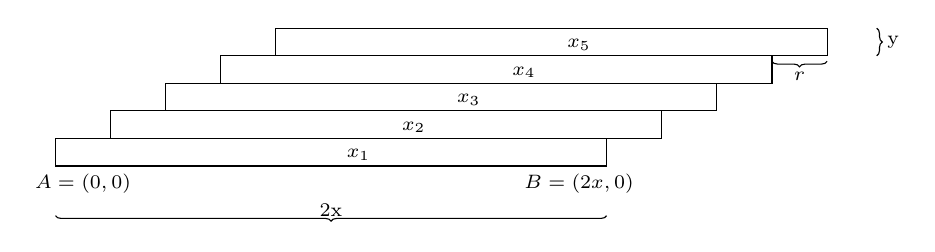
\begin{tikzpicture}[scale=0.70]
      \scriptsize \foreach \x in {1,...,5} { \draw
        (0+\x -1,0.5*\x- 0.5)--(10+\x -1,0.5*\x- 0.5)--(10+\x -1,0.5+0.5*\x- 0.5)--(0+\x- 1,0.5+0.5*\x- 0.5)--cycle;
        \node at (5+\x -1,0.25+0.5*\x -0.5)
        {$\textbullet$}; \node at (5.5+\x -1, 0.2+0.5*\x -0.5) {$ x_{\x}$ };}
      \node[below] at (0.5,0) {$A=(0,0)$}; \node[below]
      at (9.5,0) {$B=(2x,0)$}; \draw[decorate,decoration={brace,raise=2pt,amplitude=2pt,mirror}] (0,0-0.8) -- node{2x}
      (10,0-0.8) ; \draw[decorate,decoration={brace,raise=2pt,amplitude=2pt,mirror}] (14.8,2) -- node[right=3pt]{y}
      (14.8,2.5) ; \draw[decorate,decoration={brace,raise=2pt,amplitude=2pt,mirror}] (13,2) -- node[below=3pt]{$r$}
      (14,2) ;
    \end{tikzpicture}
    \label{fig:fig001}
  \end{figure}
  \begin{itemize}
    \item
          Since we just consider the horizontal component of gravity center, vertical properties can be ignored.
    \item 
          For each slab $i=1,2,\ldots,n$, the gravity center
          \begin{align}
            x_i=x+(i-1)r.
          \end{align}

    \item
          The gravity center for the entire configuration is
          \begin{align*}
            x_{c}&=\frac{1}{n}\sum_{i=1}^{n}x_i\\
                 &={1\over n} \sum_{i=1}^n(x+(i-1)r)\\
                 &={1\over n} \left[\sum_{i=1}^n x+ (\sum_{i=1}^n(i-1) )r\right]\\
                 &={1\over n} \left[nx+ {n(n-1)\over 2}r\right]\\
                 &=x+{(n-1)r\over2}.
          \end{align*}

  \end{itemize}

  
\end{frame}
\begin{frame}{1. Gravity center of slabs}
  \begin{itemize}
    \item The gravity center formula comes from
          \begin{align}
            x_c={\sum_{i=1}^n m_i x_i\over {\sum m_i}}.
          \end{align}
          for $n$ objects with mass $m_i$, gravity center $x_i$.
        
          For each slab, the mass is the same, we can denote it as $m$. Then the gravity center of the entire
          configuration is
          \begin{align*}
            x_c&={\sum_{i=1}^n m x_i\over{\sum_{i=1}^n m}}\\\tag{3}
               &={\sum_{i=1}^n m x_i\over {mn}}\\
               &={\sum_{i=1}^n x_i\over n}.
          \end{align*}
          \url{http://hyperphysics.phy-astr.gsu.edu/hbase/cm.html}
          \framebreak
    \item  Another way
          \begin{figure}[!H]
            \centering
            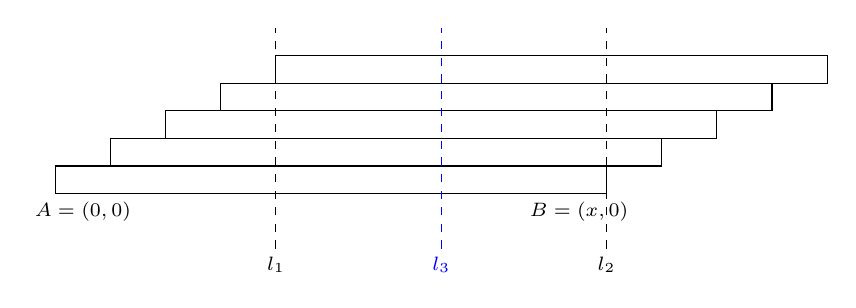
\begin{tikzpicture}[scale=0.70]
              \scriptsize \foreach \x in {0,1,...,4} { \draw
                (0+\x,0.5*\x)--(10+\x,0.5*\x)--(10+\x,0.5+0.5*\x)--(0+\x,0.5+0.5*\x)--cycle; \node at (5+\x,0.25+0.5*\x)
                {$\textbullet$}; } \node[below] at (0.5,0) {$A=(0,0)$}; \node[below] at (9.5,0) {$B=(x,0)$};
              \draw[dashed] (4,-1) node[below]{$l_1$}--(4,3); \draw[dashed] (10,-1)node[below]{$l_2$}--(10,3);
              \draw[dashed,blue] (7,-1)node[below]{$l_3$}--(7,3);
            \end{tikzpicture}
            \label{fig:fig001}
          \end{figure}
          You may note that the gravity center lies at where the left and the right sides have the equal mass.
          From the figure, the mass on the left of line $l_1$ and the right of $l_3$ equals.
          Hence the gravity center lie on the line $l_2$, the position of which is $x_{c}=(n-1)r+\frac{2x-(n-1)r}{2}=x+\frac{(n-1)r}{2}$.

        
  \end{itemize}

\end{frame}
\begin{frame}{1. Gravity center of slabs (b)}
  Check when $x_c>|AB|=2x$.  For the computation:
  \begin{align*}
    x+\frac{(n-1)r}{2}>2x\Rightarrow n>\frac{2x}{r}-1.
  \end{align*}
  \begin{itemize}
    \item for $r=5$, n>21;
    \item for $r=8$, n>13.5.
  \end{itemize}
\end{frame}





\begin{frame}{2.Number of squares}
  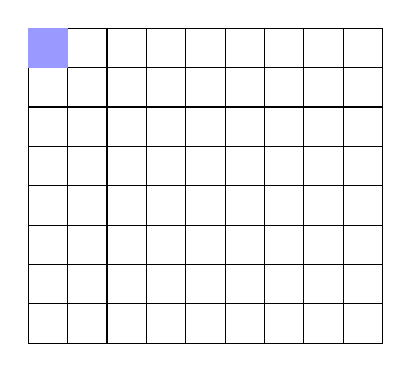
\begin{tikzpicture}[scale=0.50]
    \foreach \x in {0,...,8} { \draw (0,\x)--(9,\x); } \foreach \y in {0,...,9} { \draw (\y,0)--(\y,8); }
    \fill[blue!40!white] (0,8) rectangle (1,7);
  \end{tikzpicture}
  \begin{itemize}
    \item To counter the squares, start with a square at the top left corner of the board and move it vertically down
          and then horizontally across to account for all squares of that shape.
          \framebreak
          \begin{itemize}
            \item 1$\times$1 squares, number: $8\times 9$ 
            \item $2\times 2,\ldots, 8\times 8$ squares, number: $7\times 8,\ldots, 1\times 2$
            \item Total number:  $8\times 9+7\times 8+\cdots +1\times 2=240$
          \end{itemize}
    \item \textbf{Alternative way} A square, when projected to the sides of the grid, yield two segments of
          equal length. Conversely, a horizontal and a vertical segment of equal length,corresponds
          to a square. There are 8 vertical segments and 9 horizontal segments of length 1. Thus
          there are $8\times 9$ number of $1\times 1$ squares. Likewise, there are $7\times 8$ number of $2\times 2$ squares, etc.
    \item Number of rectangles

          Note that each rectangle corresponds uniquely to a  vertical and horizontal segment.
          \begin{itemize}
            \item Number of different horizontal segments

                  Among the 10 points, any different pair of two points corresponds a different segment, do we have
                  $\binom{10}{2}$ different choices.
            \item As above, choose two points from the 8 points. We have $\binom{9}{2}$ different choices.
            \item Totally we have $\binom{10}{2}\times \binom{9}{2}=45\times 36=240$ different choices.
          \end{itemize}

  \end{itemize}
\end{frame}
\begin{frame}{3. Number of squares (two removed)}
  \begin{wrapfigure}{r}{0.5\textwidth}
    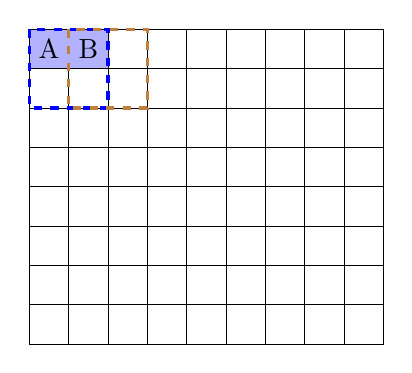
\begin{tikzpicture}[scale=0.50]
      \foreach \x in {0,...,8} { \draw (0,\x)--(9,\x); } \foreach \y in {0,...,9} { \draw (\y,0)--(\y,8); }
      \fill[blue!30!white] (0,8) rectangle (2,7); \draw (0,8) rectangle (2,7); \draw[dashed,blue,very thick] (0,8)
      rectangle (2,6); \draw[dashed,brown,very thick] (1,8) rectangle (3,6); \node at (0.5,7.5) {A}; \node at (1.5,7.5)
      {B};
    \end{tikzpicture}
  \end{wrapfigure}
  Main idea: Check how many squares in Problem 2,(a) contain the removed two squares A, B.
  \begin{itemize}
    \item Number of squares contain A or B,
          \begin{itemize}
            \item $1\times 1$: 2;
            \item $2\times 2$: 2;
            \item $\ldots$
            \item $8\times 8$: 2.
          \end{itemize}
    \item Required number of squares in incomplete chequered: 240 -16=224.       
  \end{itemize}

   
\end{frame}

\begin{frame}{4. Number of triangles}

  Find the number of triangles in each of the following figures.
  \begin{figure}[H]
    \centering
    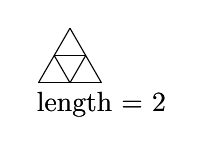
\begin{tikzpicture}[scale=0.4]
      \foreach \y in {1,...,2} { \draw (0.5*\y - 0.5, 0.866*\y- 0.866)--++ ( 3-\y , 0); \draw (\y- 1,0)--(0.5+
        0.5*\y,0.866*3- 0.866*\y); \draw (\y,0)--(0.5*\y,0.866*\y); \node[below] at (2,0) {length = 2}; }
     
    \end{tikzpicture}
    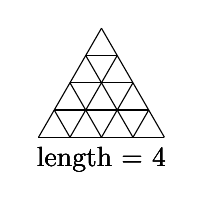
\begin{tikzpicture}[scale=0.4]
      \foreach \y in {1,...,4} { \draw (0.5*\y - 0.5, 0.866*\y- 0.866)--++ ( 5-\y , 0); \draw (\y- 1,0)--(1.5+
        0.5*\y,0.866*5- 0.866*\y); \draw (\y,0)--(0.5*\y,0.866*\y); \node[below] at (2,0) {length = 4}; }
     
    \end{tikzpicture}
    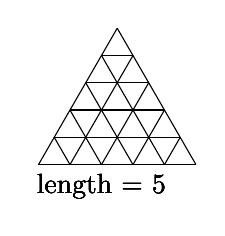
\begin{tikzpicture}[scale=0.4]
      \foreach \y in {1,...,5} { \draw (0.5*\y - 0.5, 0.866*\y- 0.866)--++ (6 -\y , 0); \draw (\y- 1,0)--(2+
        0.5*\y,0.866*6- 0.866*\y); \draw (\y,0)--(0.5*\y,0.866*\y); \node[below] at (2,0) {length = 5}; }
    \end{tikzpicture}
  \end{figure}
    
  Two type of triangles
  \begin{itemize}
    \item Up triangles $\bigtriangleup$, denote by $\bigtriangleup_k$ the up triangles of side length $k$.
    \item Down triangles $\bigtriangledown$,denote by $\bigtriangledown_k$ the up triangles of side length $k$.
  \end{itemize}

  \framebreak
  \begin{itemize}
    \item  In the first figure
          \begin{itemize}
            \item Number of up
                  triangles: $3\times \bigtriangleup_1+\bigtriangleup_2$;
            \item Number of down triangles: $\bigtriangledown_1$;
            \item Total 5 triangles.
          \end{itemize}
    \item In the second case
          \begin{itemize}
            \item $\bigtriangleup_1$:10,\quad$\bigtriangleup_2$:6,\quad$\bigtriangleup_3$:3,\quad$\bigtriangleup_4$:1;
            \item $\bigtriangledown_1$:\,\,\,6,\quad$\bigtriangledown_2$:1,\quad $\bigtriangledown_3$:0;
            \item Total 27 triangles.
          \end{itemize}
    \item In the second case
          \begin{itemize}
            \item $\bigtriangleup_1$:15,\quad$\bigtriangleup_2$:10,\quad$\bigtriangleup_3$:6,\quad$\bigtriangleup_4$:3,
                  \quad$\bigtriangleup_5$:1;
            \item $\bigtriangledown_1$:10,\quad$\bigtriangledown_2$:3,\,\,\,\quad $\bigtriangledown_3$:0;
            \item Total 48 triangles.
          \end{itemize}
          \framebreak
          
    \item Deduction for the general case
          We consider for the numbers of extra triangles of $\bigtriangleup_{n+1}$ compared to thath of
          $\bigtriangleup_{n}$
          \begin{itemize}
           \item Extra up triangles $\bigtriangleup$
                  \begin{minipage}{0.8\linewidth}
                    Add one line $l$ beneath the lowest line. Intersect the non horizontal
                    lines with l giving $n + 2$ points.
                    For each type $\bigtriangleup$ triangle, extend the two non horizontal
                    lines to intersect l at two points,
                    say A, B, with A on the left.
                    We can see that the bottom side of the triangle must lies on the line $l$. Then each pair of $(A,B)$
                    can determine an extra triangle. We have $\binom{n+2}{2}$ different pairs of $(A,B)$, thus
                    $\binom{n+2}{2}$
                    extra up triangles.
                  \end{minipage}%
                  \begin{minipage}{0.2\linewidth}
                     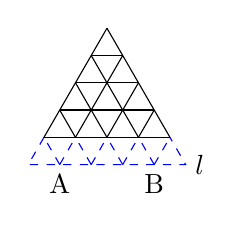
\begin{tikzpicture}[scale=0.4]
                     \foreach \y in {1,...,4} { \draw (0.5*\y - 0.5, 0.866*\y- 0.866)--++ ( 5-\y , 0); \draw (\y-
                       1,0)--(1.5+ 0.5*\y,0.866*5- 0.866*\y); \draw (\y,0)--(0.5*\y,0.866*\y); }
                      \draw[dashed,blue] (0,0)--(-0.5,-0.866)--(4.5,-0.866)--(4,0);
                      \foreach \x in {1,...,4}{   \draw[dashed,blue] (\x- 0.5,-0.866)--(\x-1,0);
                      \draw[dashed,blue] (\x- 0.5,-0.866)--(\x,0);}
                     \node[right] at (4.5,-0.886) {$l$};
                     \node[below] at (0.5,-0.886) {A};
                     \node[below] at (3.5,-0.886) {B};    
                    
                  \end{tikzpicture}
                \end{minipage}
             \framebreak
             \item Extra down triangles $\bigtriangledown$ 
                 
             
\begin{minipage}{0.7\linewidth}
                    
                  \begin{itemize}
                    \item $n=2k$ is even\\
                          We can see that each extra down triangle must satisfy that  its lowest vertex $A$ lie on the
                          line $l$.
                          With different $A$, we have $2(1+2+\cdots+k)=k(k+1)=\frac{n^2}{4}+\frac{n}{2}$ extra triangles.
                    \item $n=2k+1$ is odd\\
                          Move $A$ from left to center point (showing as the dashed line and the right side is symmetric
                          with left), we have $2(1+2+\cdots+k)+(k+1)=(k+1)^2=(\frac{n+1}{4})^2$ extra triangles.
                  \end{itemize}
                \end{minipage}%
                   \begin{minipage}{0.2\linewidth}\hspace*{2em}
                     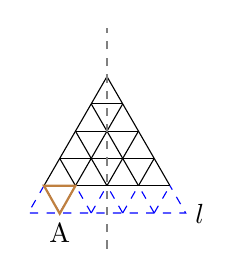
\begin{tikzpicture}[scale=0.4]
                    \foreach \y in {1,...,4} { \draw (0.5*\y - 0.5, 0.866*\y- 0.866)--++ ( 5-\y , 0); \draw (\y-
                      1,0)--(1.5+ 0.5*\y,0.866*5- 0.866*\y); \draw (\y,0)--(0.5*\y,0.866*\y); }
                      \draw[dashed,blue] (0,0)--(-0.5,-0.866)--(4.5,-0.866)--(4,0);
                      \foreach \x in {1,...,4}{   \draw[dashed,blue] (\x- 0.5,-0.866)--(\x-1,0);
                        \draw[dashed,blue] (\x- 0.5,-0.866)--(\x,0);}
                      \draw[dashed,gray] (2,-2)--(2,5);
                    \node[right] at (4.5,-0.886) {$l$};
                    \node[below] at (0.5,-0.886) {A};
                    \draw[thick,brown] (0.5,-0.886)--(0,0)--(1,0)--cycle; 
                  \end{tikzpicture}
                \end{minipage}
             \framebreak     
\item The total number of the extra triangles  is
                  
                  $\frac{3}{4}n^2+2n+1$ when $n$ is even and  $\frac{3}{4}n^2+2n+\frac{5}{4}$ when $n$ is odd, which is
                  $ \frac{3}{4}n^2+2n+1+\frac{1}{8}-\frac{(-1)^n }{8}$.
            \item The general formula of number of triangles of $\bigtriangleup_n$ is
                  \begin{align*}
                    \frac{n^3}{4}+{5n^2\over 8}+{n\over 4} -{1\over 16}+ {(-1)^{n}\over 16}.
                  \end{align*}
                  (We compute it by add extra numbers from $\bigtriangleup_1$ with the extra number formula deduced above) 

           
          \end{itemize}
          
      
  \end{itemize}

     
    

     
     
\end{frame}





\begin{frame}
  \frametitle{5. Number of squares formed by joining dots}
  \begin{minipage}{0.6\linewidth}
    Find the number of squares that can be formed by joining dots in the following diagram.
  \end{minipage}%
  \begin{minipage}{0.3\linewidth}
    \hspace*{\fill}
    \begin{tikzpicture}[scale=0.3]
      \foreach \x in {1,...,5} \foreach \y in {1,...,5}{ \fill (\x,\y) circle (2pt); }\end{tikzpicture}\hspace*{\fill}
  \end{minipage}

  \framebreak
   Type of squares:we denote $(x,y)$ by the length of square.
   \begin{itemize}
     \item (0,1),(0,2),(0,3),(0,4) i.e. Squares whose sides are vertical or horizontal.
           Showing as\\
           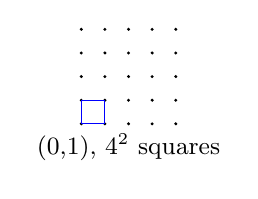
\begin{tikzpicture}[scale=0.3]
             \foreach \x in {1,...,5} \foreach \y in {1,...,5}{ \fill (\x,\y) circle (2pt); }
             \draw[blue] (2,2) rectangle (1,1);
             \node[below] at (3,1){\small (0,1),  $4^2$ squares};
           \end{tikzpicture}
           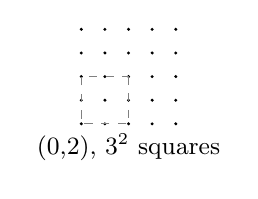
\begin{tikzpicture}[scale=0.3]
             \foreach \x in {1,...,5} \foreach \y in {1,...,5}{ \fill (\x,\y) circle (2pt); }
                         \node[below] at (3,1){\small (0,2), $3^2$ squares};
             \draw[dashed,gray] (3,3) rectangle (1,1);
           \end{tikzpicture}
           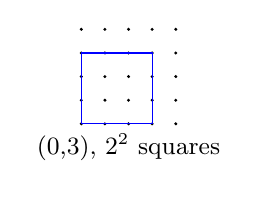
\begin{tikzpicture}[scale=0.3]
             \foreach \x in {1,...,5} \foreach \y in {1,...,5}{ \fill (\x,\y) circle (2pt); }
             \draw[blue] (4,4) rectangle (1,1);
                          \node[below] at (3,1){\small(0,3), $2^2$ squares};
           \end{tikzpicture}
            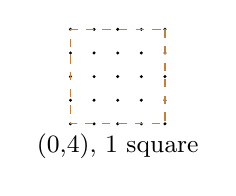
\begin{tikzpicture}[scale=0.3]
             \foreach \x in {1,...,5} \foreach \y in {1,...,5}{ \fill (\x,\y) circle (2pt); }
             \draw[dashed,brown] (5,5) rectangle (1,1);
                 \node[below] at (3,1){\small(0,4), 1 square};     
               \end{tikzpicture}

           \framebreak
           
     \item (1,1),(2,2), i.e. Squares with side length equal to $\sqrt2,\sqrt8$.\\[12pt]
            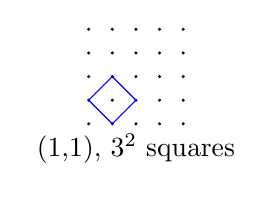
\begin{tikzpicture}[scale=0.3]
             \foreach \x in {1,...,5} \foreach \y in {1,...,5}{ \fill (\x,\y) circle (2pt); }
             \draw[blue] (2,1)--(3,2)--(2,3)--(1,2)--cycle;
             \node[below] at (3,1){(1,1), $3^2$ squares};
           \end{tikzpicture}\qquad
            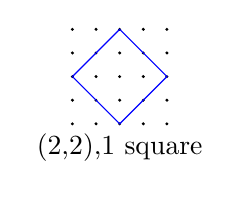
\begin{tikzpicture}[scale=0.3]
             \foreach \x in {1,...,5} \foreach \y in {1,...,5}{ \fill (\x,\y) circle (2pt); }
             \draw[blue] (3,1)--(5,3)--(3,5)--(1,3)--cycle;
             \node[below] at (3,1){(2,2),1 square};
           \end{tikzpicture}
           
     \item (1,2),(2,1),(1,3),(3,1), i.e. Squares with side length equal to $\sqrt{1^2+2^2},\sqrt{1^2+3^2}$.\\[10pt]
           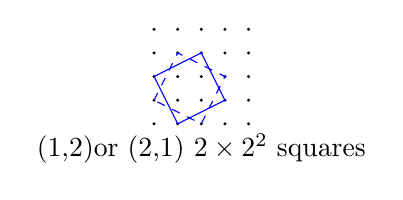
\begin{tikzpicture}[scale=0.3]
             \foreach \x in {1,...,5} \foreach \y in {1,...,5}{ \fill (\x,\y) circle (2pt); }
             \draw[blue] (2,1)--(4,2)--(3,4)--(1,3)--cycle;
             \draw[dashed,blue] (1,2)--(2,4)--(4,3)--(3,1)--cycle;
             \node[below] at (3,1){(1,2)or (2,1) $2\times 2^2$ squares};
           \end{tikzpicture}\qquad
           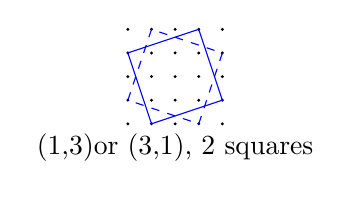
\begin{tikzpicture}[scale=0.3]
             \foreach \x in {1,...,5} \foreach \y in {1,...,5}{ \fill (\x,\y) circle (2pt); }
             \draw[blue]
             (2,1)--(5,2)--(4,5)--(1,4)--cycle;
             \draw[dashed,blue] (1,2)--(2,5)--(5,4)--(4,1)--cycle;
             \node[below] at
             (3,1){(1,3)or (3,1), 2 squares};
           \end{tikzpicture}
     \item So we have $1^2+2^2+3^2+4^2+9+1+8+2=50$ squares in all.
   \end{itemize}
\end{frame}




\begin{frame}{6.Number of Regions}
\textbf{Question:}
\begin{itemize}
	\item Draw a triangle on the plane. The plane is divided into 2 regions.
	\item Draw two triangles in the plane, what is the maximum number of regions that the plane is divided into?
	
	\item What is the answer if there are n triangles, where n  $ \geq $ 1?  
\end{itemize}
\end{frame}
\begin{frame}{6.Number of Regions}
\begin{figure}
		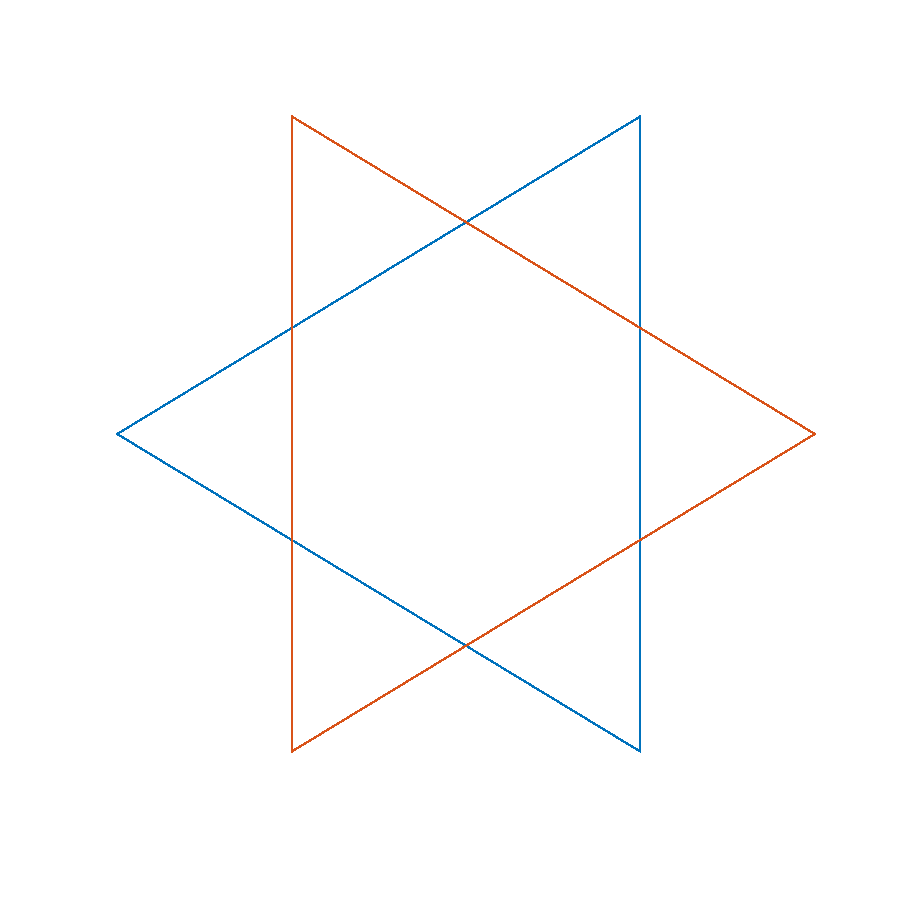
\includegraphics[width=0.49\textheight]{2.pdf}
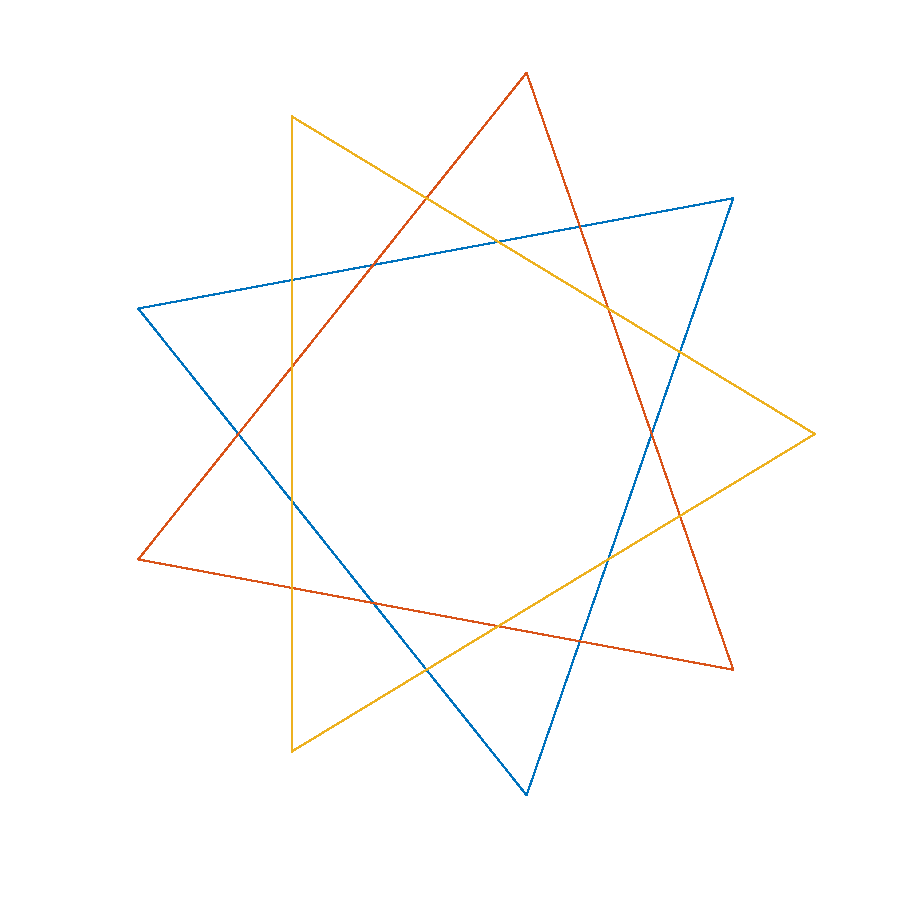
\includegraphics[width=0.49\textheight]{3.pdf}
\caption{n=2,3}
\end{figure}
Every line can intersect with most 2 edges of a trangle. Therefore, when n=2, the maximum number of regions is 8.
\framebreak
	\begin{figure}
		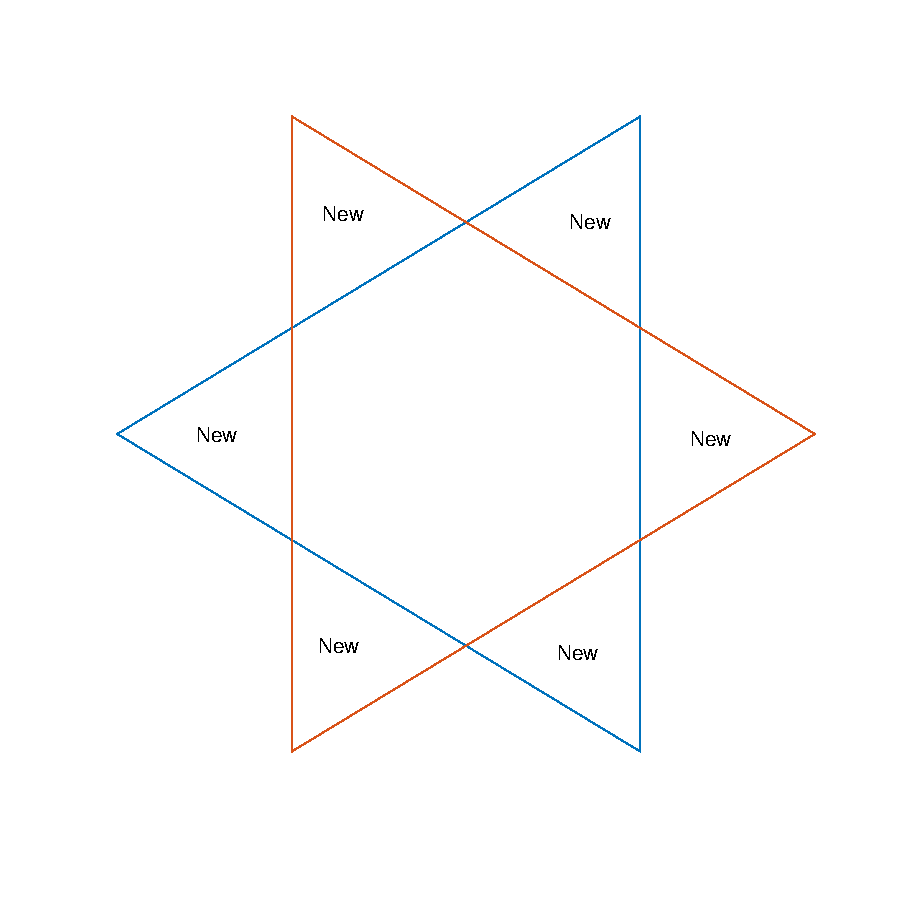
\includegraphics[width=0.5\textheight]{21.pdf}
		\caption{Counting new regions for n=2}
	\end{figure}
{ \begin{itemize}
	\item n=1, the blue triangle cut the plane into 2 regions;
	\item n=2, the orange one interscet the blue one in 6 points, Its perimeter is cut into 6 portions;
	\item Every poition of the orange curve cuts a new region form the old one. (Note: "new" is w.r.t. counting.)
\end{itemize} }
\end{frame}
\begin{frame}{6.Number of Regions}
	In $ n^{th} $ step:
	\begin{itemize}
		\item 	If the new triangle intersects an existing triangle in 6
		points, dividing the perimeter of the new triangle into 6 portions, then each portion divides an
		existing region into 2 and therefore we get 6 additional regions;
		\item  If the new triangle intersects every existing triangle in 6
		points, then the total number
		of additional regions is $ 6(n − 1) $ since there are $ n − 1 $ existing triangles.
	\end{itemize}

%\pause

 The two above condition can be satisifed:
 
  If you rotate a regualr triangle less than $ 2\pi/3 $ with its center fixed, it will interscet with a triangle in the original position in 6 points.
\end{frame}
\begin{frame}{6.Number of Regions}
	\begin{table}
		\begin{tabular}{c|c|c|c|c|c|c}
			\hline
			\# Triangle: n&0&1&2&3&$ \cdots $&n\\
			\hline
			Plus&-&1&6&12&$ \cdots $&6(n-1)\\
			\hline
			Regions&1&2&8&20&$ \cdots $&2+3n(n-1)\\
			\hline
		\end{tabular}
	\end{table}
\[2+6(1+2+3+\cdots+(n-1))=2+3n(n-1).\]
\end{frame}
\begin{frame}{6.Number of Regions}
	\begin{figure}
		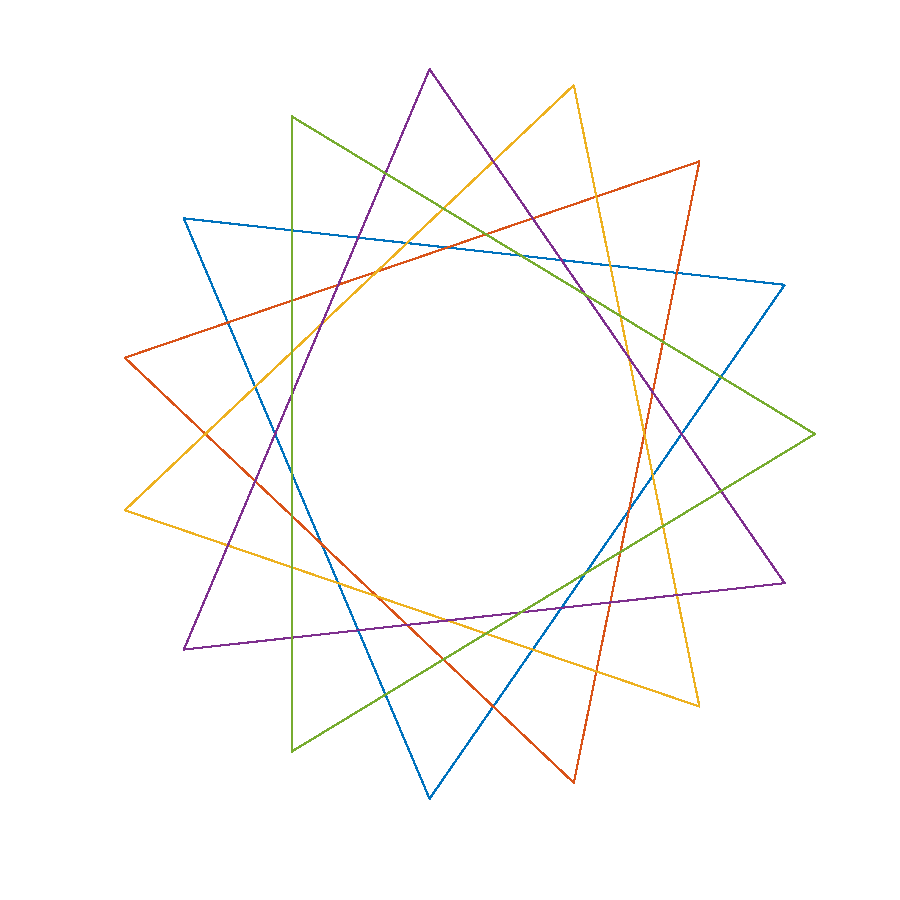
\includegraphics[width=0.49\textheight]{5.pdf}
		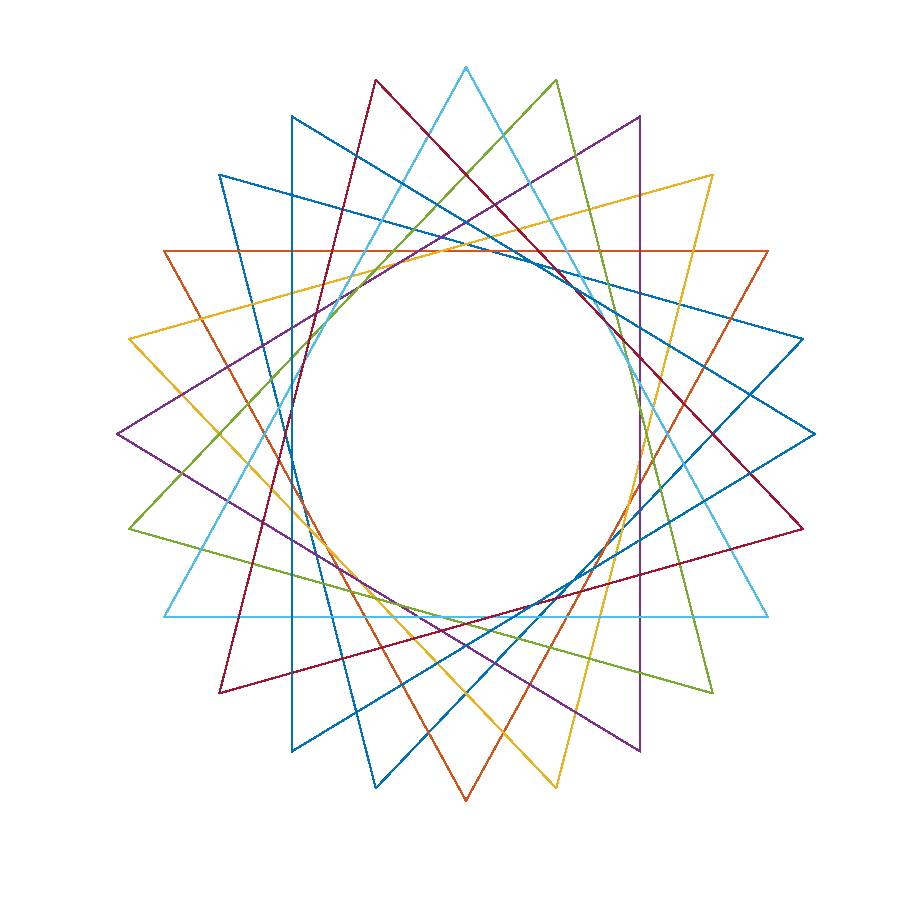
\includegraphics[width=0.49\textheight]{8.pdf}
		\caption{n=5,8}
	\end{figure}
\end{frame}
%%% Local Variables:
%%% mode: latex
%%% TeX-master: t
%%% End:



\begin{tframe}
  \vspace{8em} {\large Thank you for your listening}
\end{tframe}
\end{document}
%%% Local Variables:
%%% mode: latex
%%% TeX-master: t
%%% End:
